\documentclass[../competing_bandits_with_appendix.tex]{subfiles}
\begin{document}

\section{Introduction}\label{sec:intro}

Many modern online platforms simultaneously compete for users as well as learn from the users they manage to attract. This creates a tension between \textit{exploration} and \textit{competition}: firms experiment with potentially sub-optimal options for the sake of gaining information to make better decisions tomorrow, while they need to incentivize consumers to select them over their competitors today. For instance, Google Search and Bing compete for users in the search engine market yet at the same time need to experiment with their search and ranking algorithms to learn what works best. Similar exploration vs. competition tension arises in other application domains: recommendation systems, news and entertainment websites, online commerce, and so forth.

\OMIT{\gaedit{Bing experimenting with a ranking algorithm that ends up with a poor user experience could lead to negative short-run consequences in consumers' perceived quality of Bing and lead to more consumers choosing Google over Bing. However, this experimentation can help Bing eventually find a better ranking algorithm that would lead to positive long-run consequences in consumers' perceived quality of Bing and lead to more consumers choosing Bing over Google.}}

Online platforms routinely deploy A/B tests, and are increasingly adopting  more sophisticated exploration methodologies based on \emph{multi-armed bandits}, a well-known framework for making decisions under uncertainty and trading off exploration and exploitation (making good near-term decisions). While deploying ``better" learning algorithms for exploration would improve performance, this is not necessarily beneficial under competition, even putting aside the deployment/maintenance costs. In particular, excessive experimentation may hurt platform's reputation and decrease market share in the near term. This would leave the learning algorithms with less users to learn from, which may further degrade platform's performance relative to competitors who keep learning and improving from \emph{their} users, and so forth.

In this paper, we ask how the interplay of exploration and competition affects platforms' incentives. While some bandit algorithms are traditionally considered ``better" than others in the literature, {\bf\em does competition incentivize the adoption of the better algorithms}? How is this affected by the intensity of competition? We investigate these issues via extensive numerical experiments in a stylized duopoly model.

\xhdr{Our model.} We consider two firms that compete for users and simultaneously learn from them. Each firm commits to a multi-armed bandit algorithm, and \emph{explores} according to this algorithm. Users select between the two firms based on the current reputation score: rewards from the firm's algorithm, averaged over a recent time window. Each firm's objective is to maximize its market share (the fraction of users choosing this firm).

\tikzstyle{level 1}=[level distance=3.5cm, sibling distance=4.0cm]
\tikzstyle{level 2}=[level distance=3.5cm, sibling distance=2cm]
\tikzstyle{below} = [align=center]

\begin{figure}
\begin{center}
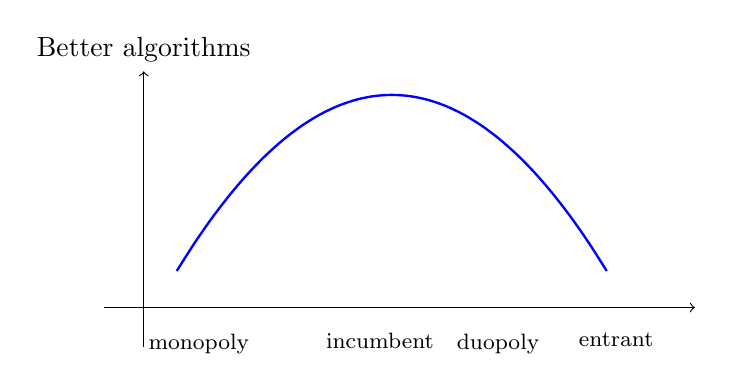
\begin{tikzpicture}
      \draw[->] (-.5,0) -- (7,0) node[right] {};
      \draw[->] (0,-.5) -- (0,3) node[above] {Better algorithms};
      \draw[scale=0.6,domain=0.7:9.8,smooth,variable=\x,blue, line width=0.3mm] plot ({\x},{4.5 - 0.18 * (\x - 5.25)^2});
     \node[below] at (0.7, -0.22) {\footnotesize monopoly};
     \node[below] at (3, -0.2) {\footnotesize incumbent};
     \node[below] at (4.5, -0.22) {\footnotesize duopoly};
     \node[below] at (6, -0.2) {\footnotesize entrant};
 \end{tikzpicture}
 \caption{A stylized ``inverted-U relationship" between strength of competition and ``level of innovation".}
\label{fig:inverted-U}
\end{center}
\end{figure}


We consider a \emph{permanent duopoly} in which both firms start at the same time, as well as \emph{temporary monopoly}: a duopoly with a first-mover. Accordingly, the intensity of competition in the model varies from ``permanent monopoly" (just one firm) to ``incumbent" (the first-mover in temporary monopoly) to permanent duopoly to ``entrant" (late-arriver in temporary monopoly).

We focus on three classes of bandit algorithms, ranging from more primitive to more sophisticated: \emph{greedy algorithms} that do not explicitly explore, algorithms that separate exploration and exploitation, and algorithms that combine the two. We know from prior work that in the absence of competition,  ``better" algorithms are better in the long run, but could be worse initially.


\xhdr{Main findings.}
We find that in the permanent duopoly, competition incentivizes firms to choose the ``greedy algorithm", and even more so if the firm is a late arriver in a market. This algorithm also prevails under monopoly, simply because it tends to be easier to deploy. Whereas the incumbent in the temporary monopoly is incentivized to deploy a more advanced exploration algorithm that performs better in the long run. As a result, we find that consumer welfare is highest under temporary monopoly and that even increasing the number of firms in the market past a duopoly makes consumers weakly worse off.

Interpreting the adoption of better algorithms as ``innovation", our findings can be framed in terms of the ``inverted-U relationship" between competition and innovation (see Figure~\ref{fig:inverted-U}). This relationship -- too little or too much competition is bad for innovation, but intermediate levels of competition tend to be better -- is a familiar theme in the economics literature, dating back to \cite{Schumpeter-42}. However, the ``inverted-U relationship'' is driven by different aspects in our model than the ones in the existing literature in economics. In our case, the barriers for innovations arise entirely from the reputational consequences of exploration in competition, as opposed to the R\&D costs (which is the more standard cause in prior work).

\xhdr{Additional findings.}
We investigate the ``first-mover advantage" phenomenon in more detail. Being first in the market gives free data to learn from (a ``data advantage") as well as a more definite, and possibly better reputation compared to an entrant (a ``reputation advantage"). We run additional experiments so as to isolate these two effects. We find that the data advantage alone can lead to a significant advantage under competition. In fact, even a small ``head start'' can get amplified into a large incumbency advantage under competition. This effect is most pronounced when the incumbent commits to a more advanced bandit algorithm. These findings suggest that competition dynamics are pertinent to the anti-trust considerations of data as a barrier to entry.

\OMIT{ %%%%%%
\swedit{Beyond the welfare implications, we also investigate the barrier to entry that follows from the incumbent's data advantage.  We run additional experiments that attempt to isolate the impact of the data advantage and reputation advantage. We find that the data advantage from the incumbent's ``small head start'' can lead to a significant incumbency advantage, especially when the incumbent commits to a more advanced bandit algorithm. Our results show that even a small degree of data asymmetry can be amplified to be a larger market advantage through competition dynamics. \gadelete{This is in contrast to the data advantage in a static environment such as discussed in \cite{varian2018artificial,bajari2018impact}, in which a small amount of additional data can only provide limited improvement in the predictive accuracy.} The effect is stronger when the incumbent commits to a more advanced bandit algorithm due to
}} %%%%%%
% in a competitive environment the relative differences in the data
% possessed by the firms may lead to a large competitive benefit due
% to the feedback loops discussed previously. In our model this effect
% is amplified when the incumbent commits to a more advanced bandit
% algorithm since, in the incumbency period, the firm gathers data on
% possible actions more efficiently leading to the relative gap upon
% entry to be larger. This is important when exploration can have
% larger reputational consequences.


\OMIT{Our findings on temporary monopoly shed light on the ``first-mover advantage" phenomenon in the digital economy. Being first in the market gives firms free data to learn from (a ``data advantage") as well as a more definite, and possibly better reputation compared to an entrant (a ``reputation advantage"). We investigate which of the two is a stronger barrier to entry. We find that both are strong barriers on their own: removing either one still gives the incumbent a substantially larger share of the market compared to the case where both are removed. However, the data advantage tends to be a stronger barrier when the incumbent commits to a more advanced bandit algorithm. One take-away is that the data advantage is not just about data quantity but also data quality.}

We also investigate how algorithms' performance ``in isolation" (without competition) is predictive of the outcomes under competition. We find that mean reputation -- arguably, the most natural performance measure ``in isolation" -- is sometimes not a good predictor. We suggest a
more refined performance measure, and use it to explain some of the competition outcomes.

While reputation scores already introduce some noise and randomness into users' choices, we consider an alternative choice model in which the noise/randomness is explicit: a small fraction of users choose a firm uniformly at random. We confirm the theoretical intuition that better algorithms prevail if the parameters -- the ``random fraction" and the time horizon -- are sufficiently large. However, we find that this effect is negligible for some smaller but still ``relevant" parameter values.

\xhdr{Discussion.}
The present paper is an experimental counterpart to \cite{CompetingBandits-itcs18}, which considered a similar duopoly model and obtained a number of theoretical results with ``asymptotic" flavor. For the sake of analytical tractability, that paper makes a somewhat unrealistic simplification that users do not observe any signals about firms' ongoing performance (instead, users choose between firms according to the firms' Bayesian-expected rewards). The high-level conclusion in \cite{CompetingBandits-itcs18} is an inverted-U relationship similar to ours, but the strength of competition is varied in a different way, using assumptions about (ir)rational user behavior.

The present paper provides a more nuanced and ``non-asymptotic" perspective. In essence, we look for substantial effects within relevant time scales. Indeed, we start our investigation by determining what time scales are relevant in the context of our model. The reputation-based choice model accounts for competition in a more direct way, allows to separate reputation vs. data advantage, and makes our model amenable to numerical simulations (unlike the model in \cite{CompetingBandits-itcs18}).

To elucidate the interplay of competition and exploration, our model is stylized in several important  respects, some of which we discuss below. Firms compete only on the quality of service, rather than, say, pricing or the range of products. Various performance signals available to the users, from personal experience to word-of-mouth to consumer reports, are abstracted as persistent ``reputation scores", which further simplified to average performance over a time window.  On the machine learning side, our setup is geared to distinguish between ``simple" vs. ``better" vs. ``smart" bandit algorithms; we are not interested in state-of-art algorithms for very realistic bandit settings.


\subsection{Related work}

\xhdr{Machine learning.} Multi-armed bandits (MAB) is a tractable abstraction for the tradeoff between exploration and exploitation. MAB problems have been studied for many decades, see \cite{Bubeck-survey12,LS19bandit-book} for background on this immense body of work; we only comment on the most related aspects.

We consider MAB with i.i.d. rewards, a well-studied and well-understood MAB model \cite{bandits-ucb1}. We focus on a well-known distinction between ``greedy" (exploitation-only) algorithms, ``naive" algorithms that separate exploration and exploitation, and ``smart" algorithms that combine them. Switching from ``greedy" to ``naive" to ``smart" algorithms involves substantial adoption costs in infrastructure and personnel training \cite{MWT-WhitePaper-2016,DS-arxiv}.

The study of competition vs. exploration has been initiated in \cite{CompetingBandits-itcs18}, as discussed above.
\OMIT{Their model differs from ours in two key respects. First, users do not see any signal about firms' past performance, and instead choose between firms according to the Bayesian-expected reward. Second, they vary the strength of competition using assumptions about (ir)rational consumer behavior, whereas we use early entry. Their results are purely theoretical; their model is amenable to proofs but not to numerical experiments. Their high-level conclusion is an inverted-U relationship between competition and innovation that is similar to ours.}
Our setting is also closely related to the ``dueling algorithms" framework \cite{DuelingAlgs-stoc11}, but this framework considers offline / full feedback scenarios whereas we focus on online machine learning problems.


In ``dueling bandits" (e.g., \cite{Yue-dueling-icml09, Yue-dueling12}), an algorithm sets up a ``duel" between a pair of arms in each round, and only learns which arm has ``won". While this setting features a form of competition inside an MAB problem, it is very different from ours.


The interplay between exploration, exploitation and incentives has been studied in other scenarios: incentivizing exploration in a recommendation system,
    \eg \cite{Kremer-JPE14,Frazier-ec14,Che-13,ICexploration-ec15,Bimpikis-exploration-ms17},
dynamic auctions
    (see \cite{DynAuctions-survey10} for background),
online ad auctions, \eg
    \cite{MechMAB-ec09,DevanurK09,NSV08,Transform-ec10-jacm},
human computation
    \cite{RepeatedPA-ec14,Ghosh-itcs13,Krause-www13},
and repeated auctions, \eg
    \cite{Amin-auctions-nips13,Amin-auctions-nips14,Jieming-ec18}.


\xhdr{Economics.}
Our work is related to a longstanding economics literature on competition vs. innovation, \eg \cite{Schumpeter-42,barro2004economic,Aghion-QJE05}. While this literature focuses on R\&D costs of innovation, ``reputational costs" seem new and specific to exploration.


Whether data gives competitive advantage
has been studied theoretically in \cite{varian2018artificial,
  lambrecht2015can} and empirically in
\cite{bajari2018impact}.
While these papers find that small amounts
  of additional data do not provide significant improvement,
 % in training a more predictive model,
  they focus on learning in isolation.
  %, which overlooks certain aspects in a competition.
%\swdelete{These studies consider the effect of additional data in terms of helping towards solving a machine learning problem in isolation and argue that it does not play a large role.}
We ask how additional data helps when firms simultaneously solve a machine learning problem and compete for consumers. Due to the competition dynamics in our model, we find that even a small amount of additional data tends to help a lot. The first-mover advantage has been well-studied in other settings in economics and marketing, see survey \cite{kerin1992first}.


\end{document}
%%% Local Variables:
%%% mode: latex
%%% TeX-master: "../competing_bandits"
%%% End:
